
\chapter{Mise en \oe{}uvre de \PpFf}
\label{implementation.chap}


Ce chapitre pr\'esente une description d\'etaill\'ee de la fa\c{c}on dont \TT{PpFf} est impl\'ement\'e. 
%
De fa\c{c}on g\'en\'erale, la mise en \oe{}uvre est bas\'ee sur la biblioth\`eque \TT{FastFlow}, h\'eritant et \'etendant plusieurs de ses classes. Ce chapitre est divis\'e dans deux sections.

La premi\`ere section d\'ecrit les diff\'erents modules composant la biblioth\`eque \TT{PpFf} et la deuxi\`eme section pr\'esente la description de plusieurs exemples complets d\'ecrivant comment un programme \PpFf{} est compil\'e et ex\'ecut\'e.


\section{Les \'el\'ements de \TT{PpFf}}

\begin{figure}
\centering
     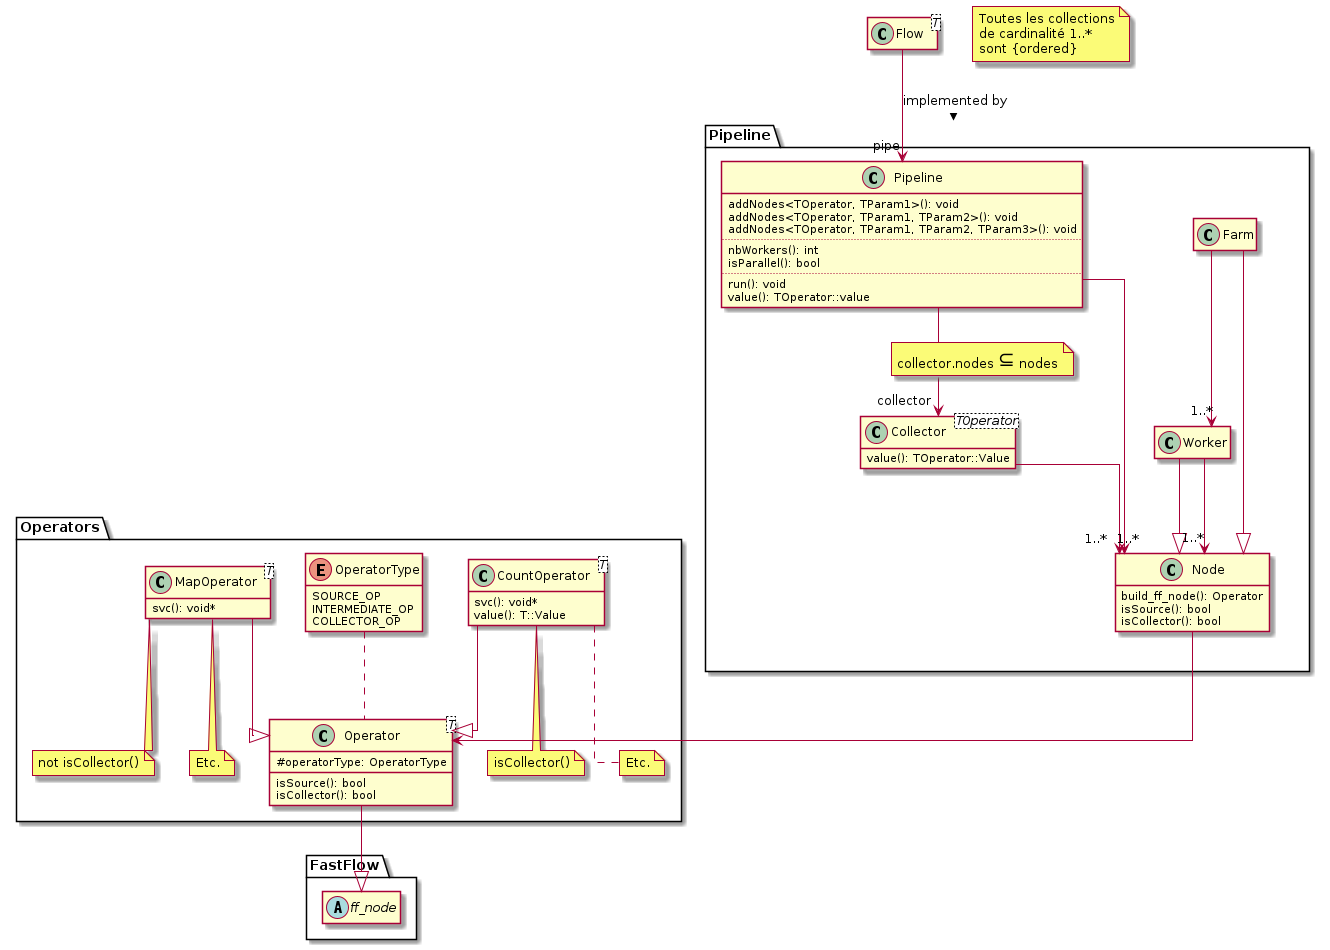
\includegraphics[width=1.0\textwidth]{Figures/all.png}
      \caption{Les modules de \TT{PpFf}.}
       \label{All.fig}
\end{figure}

La biblioth\`eque \TT{PpFf} est compos\'ee de plusieurs modules qui permettent de g\'erer le traitement de donn\'ees. Une vue d'ensemble de ces modules est illustr\'ee dans la figure~\ref{All.fig}.

\begin{itemize}

\item Le point d'entr\'ee de \ppff\ est la classe \TT{Flow}, avec laquelle interagissent les d\'eveloppeurs pour cr\'eer des flux de traitement. Toutes les op\'erations de traitement d'un flux de \TT{PpFf} sont li\'ees aux m\'ethodes expos\'ees par cette classe. 

\item Le c\oe{}ur du traitement de \TT{PpFf} est le module \TT{Pipeline}. La cr\'eation et l'ex\'ecution d'un flux sont g\'er\'ees par celui-l\`a. 

\item Dans le module \TT{Operators}, on retrouve tous les op\'erateurs d\'efinis dans \TT{PpFf}. Expos\'es \`a l'utilisateur par le biais de l'\TT{API} de \TT{PpFf}, ces op\'erateurs permettent de traiter les donn\'ees.

\item Le dernier module, \TT{FastFlow}, est la biblioth\`eque au–dessus de laquelle \TT{PpFf} est impl\'ement\'e.


\end{itemize}

\subsection{Flow}

\begin{figure}
\centering
     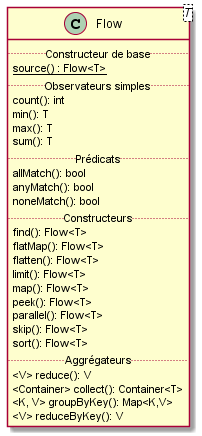
\includegraphics[width=0.5\textwidth]{Figures/flow.png}
      \caption{Les diff\'erentes m\'ethodes export\'ees par l'API de \TT{PpFf}.}
       \label{Flow.fig}
\end{figure}

\TT{Flow} est l'\TT{API} de la biblioth\`eque \TT{PpFf}, l'interface avec laquelle interagit le d\'eveloppeur. La figure~\ref{Flow.fig} pr\'esente une vue d'ensemble des diverses m\'ethodes export\'ees par \TT{PpFf}. Selon le type export\'e par l'\TT{API}, les m\'ethodes sont divis\'ees en plusieurs groupes : Constructeur de base, Observateurs simples, Pr\'edicats et Agr\'egateurs.

Constructeur de base est le groupe qui permet de d\'efinir un flux de donn\'ees. En g\'en\'eral ce groupe combine les m\'ethodes qui fournissent les donn\'ees au flux. Sans un appel \`a une telle m\'ethode, un flux ne peut pas exister. Le deuxi\`me groupe du \TT{Flow}, Observateurs simples, est le groupe qui combine les m\'ethodes qui retournent une seule valeur. Un autre groupe de \TT{Flow} o\`u les m\'ethodes retournent une seule valeur est le groupe Pr\'edicate. Par rapport au Observateurs simples, les m\'ethodes de ce groupe retournent une valeur qui peut \^etre vraie ou fausse. Les m\'ethodes du troisi\`eme groupe de \TT{Flow}, Constructeurs, retournent une r\'ef\'erence vers l'objet \TT{Flow}. Ce m\'ecanisme permet d'encha\^iner les m\'ethodes de l'\TT{API}. Le dernier groupe de \TT{Flow}, Agr\'egateurs, rassemble les m\'ethodes d'agr\'egation de l'\TT{API}. La valeur retourn\'ee par ces m\'ethodes peut \^etre une valeur simple (par ex., r\'esultat bool\'een ou entier) ou une collection de valeurs.

L'\TT{API} de \TT{PpFf} permet d'appliquer plusieurs op\'erations en m\^eme temps sur une collection de donn\'ees. Ceci est possible en encha\^inant les m\'ethodes. Les m\'ethodes de l'\TT{API} peuvent \^etre enchain\'ees tant qu'elles retournent une r\'ef\'erence \`a \TT{Flow}. Lorsqu'une m\'ethode retourne une valeur, le traitement de donn\'ees sera ex\'ecut\'e. 


\begin{lstlisting}[
label={count.c++},
language=c++,
caption={Des extraits du code de la m\'ethode count de l'API de \TT{PpFf}. },
frame=single,
float]
    // ...

	typedef CountOperator<int> Count;
            
	pipe.addNodes<Count>(pipe.nbWorkers());
	pipe.run();

	return pipe.value<Count, int>();


    // ...
\end{lstlisting}

L'\TT{API} de \TT{PpFf} a \'et\'e con\c {c}u pour \^etre simple \`a utiliser en cachant la complexit\'e des m\'ecanismes concurrents utilis\'es. Il ne fait que d\'el\'eguer la cr\'eation et l'ex\'ecution du flux au module \TT{Pipeline}. Des extraits du code de la m\'ethode \TT{count} sont pr\'esent\'es dans le listing~\ref{count.c++}. L'objet \TT{pipe}, une instance de la classe \TT{Pipeline}, cr\'ee et ajoute les op\'erateurs du type \TT{Count} dans le flux en appelant la m\'ethode \TT{addNodes}. Une fois le traitement ex\'ecut\'e en appelant la m\'ethode \TT{run}, \TT{pipe} retourne la valeur du type entier sp\'ecifi\'e dans le deuxi\`eme param\`etre template de la m\'ethode \TT{value}.

\subsection{Pipeline}
\subsection{Operateurs}


\section{Impl\'ementation de \TT{PpFf} avec \TT{FastFlow} : un exemple}


\begin{itemize}

\item objets1 

\item objets2 

\item objets3 


\end{itemize}
